\documentclass[a4paper]{article}
%\usepackage[singlespacing]{setspace}
\usepackage[onehalfspacing]{setspace}
%\usepackage[doublespacing]{setspace}
\usepackage{geometry} % Required for adjusting page dimensions and margins
\usepackage{amsmath,amsfonts,stmaryrd,amssymb,mathtools,dsfont} % Math packages
\usepackage{tabularx}
\usepackage{colortbl}
\usepackage{listings}
\usepackage{amsmath}
\usepackage{amssymb}
\usepackage{enumerate}
\usepackage{enumitem}
\usepackage{amsthm}
\usepackage{subcaption}
\usepackage{float}
\usepackage[table,xcdraw]{xcolor}
\usepackage{tikz-qtree}
\usepackage{forest}
\usepackage{changepage,titlesec,fancyhdr} % For styling Header and Titles
\pagestyle{fancy}
\usepackage{pgfplots}
\renewcommand{\headrulewidth}{0.5pt} % Linienbreite anpassen, falls gewünscht
\renewcommand{\headrule}{
    \makebox[\textwidth]{\rule{1.0\textwidth}{0.5pt}} 
}
\usepackage{amsmath}
\pagestyle{fancy}
\usepackage{diagbox}
\usepackage{xfrac}

\usepackage{enumerate} % Custom item numbers for enumerations

\usepackage[ruled]{algorithm2e} % Algorithms

\usepackage[framemethod=tikz]{mdframed} % Allows defining custom boxed/framed environments

\usepackage{listings} % File listings, with syntax highlighting
\lstset{
	basicstyle=\ttfamily, % Typeset listings in monospace font
}

\usepackage[ddmmyyyy]{datetime}


\geometry{
	paper=a4paper, % Paper size, change to letterpaper for US letter size
	top=3cm, % Top margin
	bottom=3cm, % Bottom margin
	left=2.5cm, % Left margin
	right=2.5cm, % Right margin
	headheight=25pt, % Header height
	footskip=1.5cm, % Space from the bottom margin to the baseline of the footer
	headsep=1cm, % Space from the top margin to the baseline of the header
	%showframe, % Uncomment to show how the type block is set on the page
}
\lhead{\vspace{0.5\baselineskip}Übungsblatt 1}
\chead{\bfseries{Einführung in Verteilte Systeme\\Sommersemester 2025}}
\rhead{\vspace{0.5\baselineskip}Werner, 7987847}
\fancyheadoffset[R]{0cm}

\begin{document}
\setcounter{section}{1}
\subsection{}
Es sollen Daten über eine Netzwerkverbindung von Frankfurt nach New York übertragen werden.
\begin{itemize}
    \item Fall A: Die Daten werden durch ein Transatlantikkabel übertragen. Die Signalausbreitungs-\\
    geschwindigkeit im Kabel betrage $c_k$ = 200 000 km/s.
    \item Fall B: Ein geostationärer Kommunikationssatellit übertrage die Daten. Geostationäre Satelliten befinden sich auf einer Flughöhe von ca. 36 000 km über der Erdoberfläche. Der benutzte Satellit befinde sich auf halber Strecke zwischen Europa und den USA (Längengrad ca. $30^\circ$ West; Sie dürfen die Erdkrümmung bei dieser Aufgabe vernachlässigen). Die Signalausbreitungsgeschwindigkeit in der Luft bzw. im Vakuum betrage $c$ = 300 000 km/s.
\end{itemize}
Die Distanz (Luftlinie) zwischen den beiden Städten beträgt ca. 6300 km. Nehmen Sie vereinfachend an, dass weder dazwischenliegende Router noch die Endstellen selbst Latenz hinzufügen. Die Datenrate betrage in beiden Fällen 10 Gbit/s.
\begin{enumerate}[label=\alph*)]
    \item Schätzen Sie die bestmögliche Round-Trip-Latenz der Kabelverbindung (Fall A).\\\\
    Die One-Way Latenz lautet:
    \[
    \frac{6.300 km}{200.000 km/s}=0,0315 s = 31,5 ms
    \]
    Die Round-Way Latenz lautet dann:
    \[
    L_A = 2 \cdot 31,5 ms = 63 ms
    \]
    \item Schätzen Sie die bestmögliche Round-Trip-Latenz der Satellitenverbindung (Fall B).\\\\
    Wir berechnen mit Pythagoras (Höhe h des Sateliten zur Erde und Distanz d der beiden Städte zueinander):
    \[
        d_{Sat}=\sqrt{h^2+\left(\frac{d}{2}\right)^2}=\sqrt{(36.000km)^2+\left(\frac{6300km}{2}\right)^2}\approx36.137,5 km
    \]
    Demnach ist die Round-Way Distanz:
    \[
    L_B=\frac{d_{Sat}\cdot 4}{300.000km/s}=\frac{144.550 km}{300.000km/s}=0,4818 s = 481,8 ms
    \]
    \item Es soll nun ein ganzer Verzeichnisbaum mit einzelnen Dateien von jeweils 50 MB Größe übertragen werden. Die Übertragung der nächsten Datei erfolgt erst, nachdem eine Datei vollständig übertragen und der Empfang dem Sender bestätigt wurde. Was sind die effektiven Übertragungsraten für Kabel- und Satellitenverbindung?\\\\
    Die Datenrate lautet:
    \[
    \frac{50 mbyte}{10 Gbit/s}=\frac{0,4Gbit}{10 Gbit/s}=0,04 s = 40 ms
    \]
    Somit ist die Dauer ein Datenpaket von 50MB zu verschicken, welche weitere Pakete währenddessen blockiert dann:
    \[
    L'_A=63 ms + 40 ms = 103 ms
    \]
    Bei der Satelitenverbindung:
    \[
    L'_B=481,8 ms + 40 ms = 521,8 ms
    \]
    Nach In-betrachtnahme dieser Blockade, ist die effektive Übertragunsgrate:
    \[
    E_A=\frac{50 mbyte}{L'_A}=\frac{50 mbyte}{0,103 s}=485,4 \frac{mbyte}{s}=3,88 Gbit/s
    \]
    und bei der Satelitenverbindung:
    \[
    E_B=\frac{50 mbyte}{L'B}=\frac{50 mbyte}{0,5218 s}=766,6\frac{mbyte}{s}=0,7666 Gbit/s
    \]
\end{enumerate}

\subsection{}
Mit dem ping Programm können Sie ein Testpacket an einen bestimmten Ort senden und prüfen wie lange es dorthin und wieder zurück braucht.
\begin{enumerate}[label=\alph*)]
    \item Testen Sie mit ping wie lange eine Datenübertragung von Ihrem Standort zu anderen Standorten benötigt. Benutzen Sie hier uni-frankfurt.de, cern.ch, berkeley.edu, stanford.edu, www.kek.jp
    \begin{figure}[H]
        \centering
        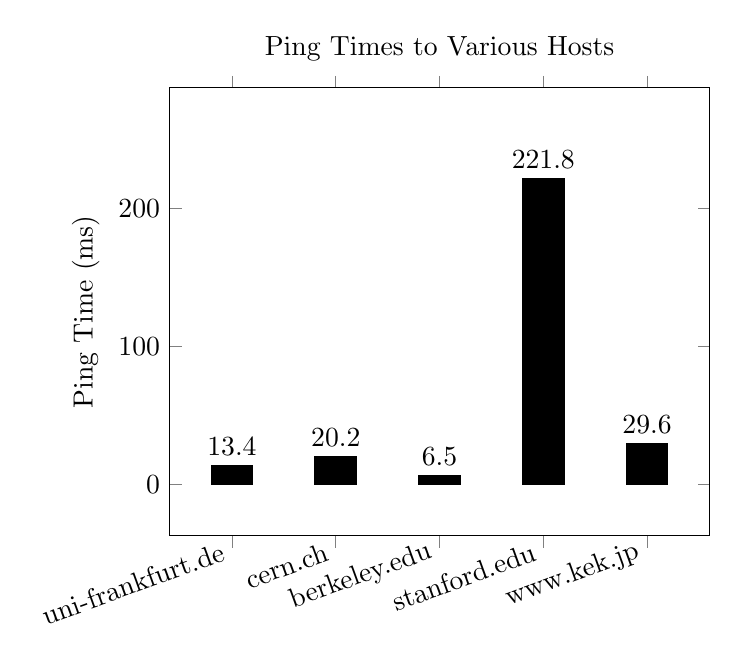
\begin{tikzpicture}
            \begin{axis}[
                ybar,
                bar width=15pt,
                ylabel={Ping Time (ms)},
                symbolic x coords={uni-frankfurt.de, cern.ch, berkeley.edu, stanford.edu, www.kek.jp},
                xtick=data,
                x tick label style={rotate=20, anchor=east},
                ymin=0,
                ymax=250,
                nodes near coords,
                enlargelimits=0.15,
                title={Ping Times to Various Hosts}
            ]
            \addplot[
            fill=black, 
            draw=black,
            mark=none
            ] coordinates {
                (uni-frankfurt.de, 13.4)
                (cern.ch, 20.2)
                (berkeley.edu, 6.5)
                (stanford.edu, 221.8)
                (www.kek.jp, 29.6)
            };
            \end{axis}
        \end{tikzpicture}
    \end{figure}
    \item Zeichen Sie anhand der Daten die Übertragungszeit über das Internet als Funktion der Entfernung auf.\\\\
    \begin{center}
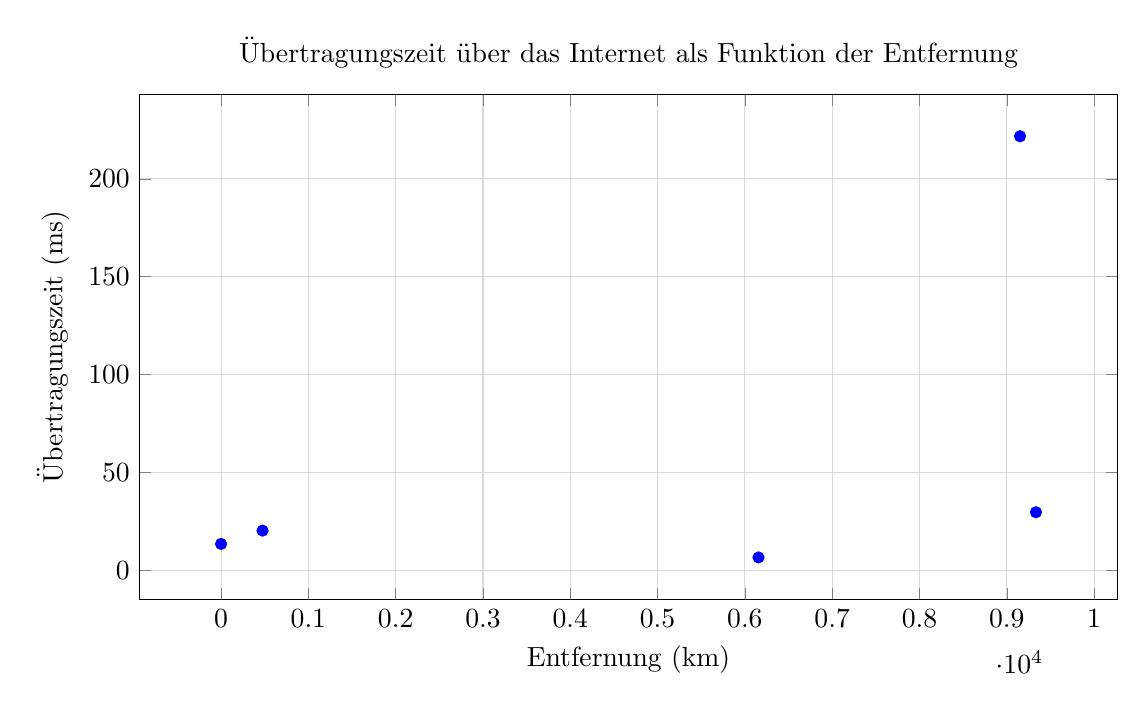
\begin{tikzpicture}
\begin{axis}[
    width=14cm,
    height=8cm,
    grid=both,
    xlabel={Entfernung (km)},
    ylabel={Übertragungszeit (ms)},
    title={Übertragungszeit über das Internet als Funktion der Entfernung},
    enlargelimits=true,
    xtick distance=1000,
    ytick distance=50,
    minor tick style={draw=none},
    every major grid/.style={gray!30},
    every minor grid/.style={gray!10},
]

\addplot[
    only marks,
    mark=*,
    color=blue,
] coordinates {
    (0, 13.4)
    (475, 20.2)
    (6156, 6.5)
    (9152, 221.8)
    (9334, 29.6)
};

%\addplot[
%    smooth,
%    thick,
%    red,
% ]
 coordinates {
    (0, 13.4)
    (475, 20.2)
    (6156, 6.5)
    (9152, 221.8)
    (9334, 29.6)
};

\end{axis}
\end{tikzpicture}
\end{center}
    \item Diskutieren Sie die Ergebnisse aus b).\\\\
    Zunächst muss verstanden werden, dass die Ergebnisse nur lokale Werte sind, die von jeder anderen Position zu jedem anderen Zeitpunkt anders sein können.\\
    Der Ping zu servern hängt von so vielen Faktoren ab, dass dies kaum vorhergesagt werden kann.\\
    Der Ausschlag von der Stanford-Domain kann zum Beispiel daher kommen, dass der Server in dem Moment oder generell langsamer ist und länger braucht um den Ping zurückzuschicken. Der Ping zur Japanischen Webseite ist deutlich geringer als zunächst erwartet würde, dies liegt daran, dass die Seite auf einem Hosting-Provider (in diesem Fall AWS, was durch den \texttt{ping} command erkannt werden kann) gehostet wird welcher auch Server in Europa hat. Somit wird bei dem DNS Request der domain die nähere, europäische IP resolved.
\end{enumerate}
\end{document}
